% All parts removed from the thesis that might be relevant after all.

\subsection{Indirect Testing}
\emph{Unit test that tests a production method through at least one intermediate method.}\\

An indirect test uses an intermediate object to bring the SUT in the correct state. We can formally define an indirect test, by first defining some parameters:

$\begin{array}{ll}
t &  \hbox{test method} \\
p &  \hbox{production method} \\
C(t) & \hbox{tested class of } t \\
P  & \hbox{Set of Production classes} \\
T & \hbox{Set of Test classes} \\
uses(m_1,m_2) & \hbox{There is a method invocation from $m_1$ to $m_2$} \\
\end{array}$ \\

A test $t$ has an indirect test smell, if there exists a chain of method calls from $t$ to a method $m \in C(t)$ with at least one intermediate method $w$. Formally: \\

\begin{math} 
Indirect(t) : \exists_w : t \rightarrow ... \rightarrow w \rightarrow ... \rightarrow p \wedge p \in C(t), w \notin C(t) 
\end{math}

Where $ m_1 \rightarrow m_2$ is shorthand for $uses(m_1, m_2)$ \\

\todo{update this description}
In Figure \ref{fig:IndirectTest} test class $TC1$ contains two test methods $t$ and $u$. The tested class is $PC1$. In this example, test $u$ is an indirect test, for it calls method $c$ in class $PC2$ to bring the SUT in the correct state. Methods from the tested class are accessed through class $PC2$. 

\begin{figure}[!ht]
	
	\centering
	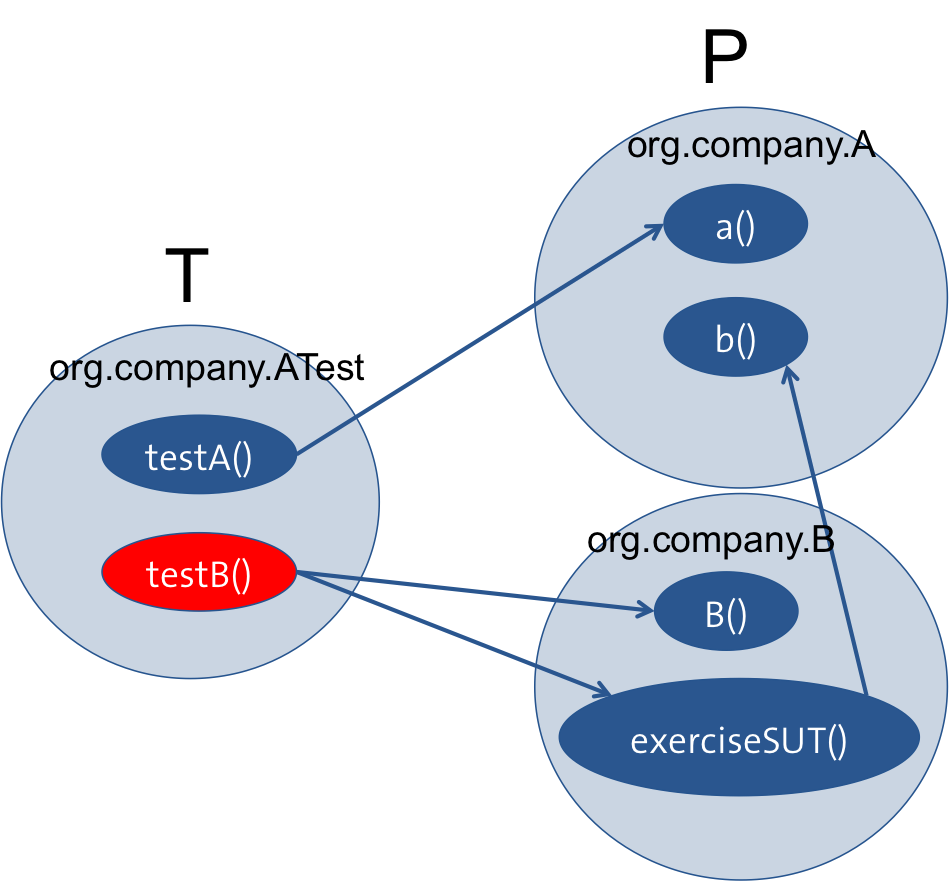
\includegraphics[width=0.5\textwidth]{figures/IndirectTest.png}
	\caption{In red an indirect test with weight 1}
	\label{fig:IndirectTest}
\end{figure}

\subsubsection{Obtain tested class}
\todo{via formalization framework, use general approach of SAT call-resolving. If implemented, change description!}
To obtain the tested class we map test classes and production classes in the same package to each other, relying on the convention that these are placed in the same package, and both class names start the same. Sometimes developers make multiple test classes to test the same production class, but with different intentions. For example: \texttt{[path].MixedNeo4jRepositoriesAutoConfigurationTests} tests the class  \texttt{[path].Neo4jRepositoriesAutoConfiguration}. In Java a class can have inner classes. We chose to not look at inner classes and mapped a test class always to the base class, when inner classes where concerned. The test class \texttt{ResourceServerTokenServicesConfigurationTests.Customizer} would be mapped to  \texttt{ResourceServerTokenServicesConfiguration}. 

We then check if the test class name starts with the production class name. Inner classes are eliminated from the string similarity check as described above. In order to catch subtle differences in class names (MixedNeo4j(..) vs Neo4j(..))we use a String similarity measure, in particular n-grams. . N-grams have proven to be a good string similarity measure in finding source code refactorings. The way n-grams work is chopping up a string in buckets, using a sliding window of length $n$. The buckets of two strings are checked for equality, resulting in a percentage of matches. We experimentally chose 75\% as a threshold. Above this threshold, two strings are considered 'matched'. Since class names are generally very long, the accuracy of using n-grams really high. Note that we calculate the string similarity for class names, without the package prefix, and inner-class postfix. \todo{determine real accuracy}

To see the effect of n-grams consider the task of matching the test class

\texttt{MixedNeo4jRepositoryAutoConfiguration}

to two potential production classes

\texttt{Neo4jRepositoriesAutoConfiguration} and

\texttt{Neo4jRepositoriesAutoConfigureRegistrar}. 

Using a sliding window of 2, we get 86\% for the first production class and 64\% for the second.  


\subsection{For Testers Only}
\emph{Production class of which methods are only invoked by methods in test code.}\\

When a production class is only used by test methods, we label it For Testers Only (FTO), formally: \\

\begin{math}
\forall l,m; m \in P_i \wedge l \in T \wedge l,m \in \{method\} : uses(l, m)
\end{math} \\

When reading the code of a FTO class, it is not clear that this class is only used by test methods. When a developer changes a FTO class, he does not have the affected test methods in mind. Test failures as a result of changing a FTO class might then come as a surprise. See Figure \ref{fig:FTO} for a visual example. Class $A$ is being used by a method in class $B$, which is a production class, so not a FTO class. Class $B$ however, is only used by methods in test code.

\begin{figure}[!ht]
	
	\centering
	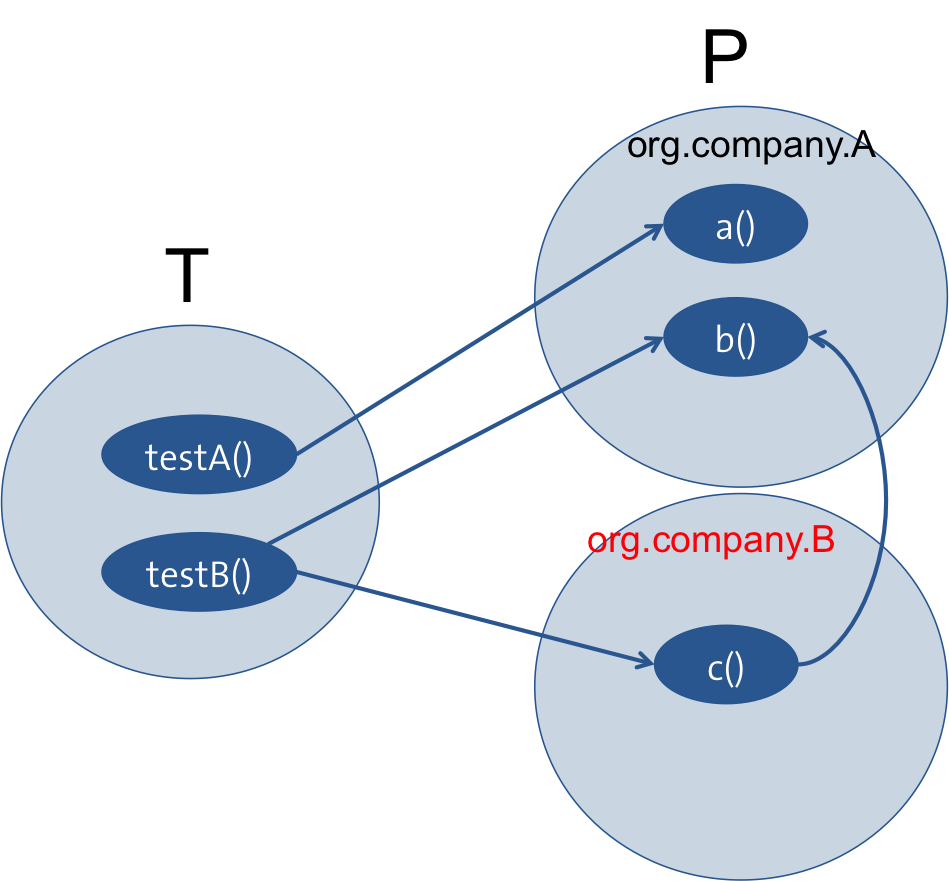
\includegraphics[width=0.5\textwidth]{figures/FTO.png}
	\caption{Class B is a FTO class}
	\label{fig:FTO}
\end{figure}